\section{Cluster aspects of Lagrangian fillings}

The object of this last section is to bring together the cluster algebra structure on $\Z[X(\beta)]$ and the symplectic topology of $\La_\beta$ and its Lagrangian fillings $L_\w$ arising from Demazure weaves $\wb$. First, in \Cref{ssec:torus_Lagrangian_filling_from_weave} we describe the torus $T_\w\sse X(\beta)$ underlying a cluster seed in terms of the symplectic topology of $L_\w$, and interpret the associated $\SA$ and $\SX$-lattices with their intersection forms via the algebraic topology of $L_\w$. Second, the symplectic construction of the corresponding cluster $\SA$ and $\SX$-variables is presented in \Cref{ssec:X_coordinates_Lagrangian_filling_from_weave}, and \Cref{ssec:cluster_mutation_Lagrangian_filling_from_weave} explains the relation between Lagrangian disk surgeries and weave and cluster mutations.
%%%%%%%%%%%%%%%%%%%%%%%%%%%%%%%%%%%%%%%%%%%%%%%%%%%%%%%%
%%%%%%%%%%%%%%%%%%%%%%%%%%%%%%%%%%%%%%%%%%%%%%%%%%%%%%%%
%%%%%%%%%%%%%%%%%%%%%%%%%%%%%%%%%%%%%%%%%%%%%%%%%%%%%%%%
\subsection{The torus $T_\w$ associated to the Lagrangian filling $L_\w$}\label{ssec:torus_Lagrangian_filling_from_weave} Let $\beta\in\brn$ be a positive braid word and $X(\beta)$ its braid variety. Consider a Demazure weave $\w:\beta\to\delta(\beta)$. By \Cref{cor:weave_to_toric_embedding}, specifically \eqref{eq:weave_tori_map}, there exists an open embedding
$$\iota_\w:(\bG_m)^d\hookrightarrow X(\beta).$$
\noindent Independently, \Cref{prop:torus_from_filling} or \eqref{eq:cobordism_map} applied to the Lagrangian filling $L=L_\w$ provides an open inclusion
\begin{equation}\label{eq:Floer_torus}
\Spec(\hH_0(\varepsilon_{L_\w})):\Spec(\Z[\hH_1(L_\w,\tt;\Z)])\hookrightarrow \Spec\mbox{H}_0(\mathbb{A}^{ab}(\La_{\beta}))
\end{equation}
of algebraic varieties over $\Z$. \Cref{lem:floer_morphisms_weave_morphisms} and \cite[Section 5]{CasalsNg22} imply the following:
\begin{proposition}\label{prop:weave_tori_and_Lagrangian_fillings}
In the notation above, there exists a commutative diagram
\[
\begin{tikzcd}
    \Spec(\Z[\hH_1(L_\w,\tt;\Z)]) \arrow[r, hook,"\eqref{eq:Floer_torus}"] \arrow[d, "\tiny\mbox{id}"'] & \Spec(\hH_0(\mathbb{A}^{ab}(\La_\beta))) \arrow[d, "\mbox{\tiny\Cref{thm:braid_varieties_from_Legendrian}.(i)}","\cong"
'] \\
    T_\w \arrow[r, hook,"\iota_\w"',"\eqref{eq:weave_tori_map}"] & X(\beta)
\end{tikzcd}
\]
In particular, $\operatorname{im}(\Spec(\hH_0(\varepsilon_{L_\w})))=\operatorname{im}(\iota_\w)$
as open toric charts in $X(\beta)$.\sbs
\end{proposition}
\noindent \Cref{prop:weave_tori_and_Lagrangian_fillings} states that the Floer-theoretic toric chart associated to $L_\w$ coincides with the toric chart $T_\w\sse X(\beta)$ constructed via the weave $\w$ using the transversality conditions on flags given by $\w$, cf.~\Cref{ssec:weave_tori_braid_varieties}. The identification of the weave torus $T_\w$ with $\Spec(\Z[\hH_1(L_\w,\tt;\Z)])$ allows us to give a symplectic geometric description of the points in $T_\w$, as follows.\\

\noindent The $R$-points of the algebraic variety $\Spec(\Z[\hH_1(L_\w,\tt;\Z)])$, where $R$ is a commutative ring, are given by
\begin{equation}\label{eq:points_of_Tw}
\mbox{Hom}_{\Z-\mbox{alg}}(\Z[\hH_1(L_\w,\tt;\Z)],R)\cong \mbox{Hom}_{\Z-\mbox{mod}}(\hH_1(L_\w,\tt;\Z),R^\times)\cong \hH^1(L_\w,\tt;R^\times)
\end{equation}

\noindent Consequently, \color{blue}the $R$-points of a weave torus $T_\w\cong \Spec(\Z[\hH_1(L_\w,\tt;\Z)])$ parametrize isomorphism classes of rank-one $R$-local systems on the surface $L_\w$, with a common trivialization of the stalks at $\tt$\color{black}. Indeed, this follows from the isomorphism $H_1\cong \pi_1^{ab}$, and the stalks must be isomorphic to the rank-one free $R$-module $R$ because $R^\times\cong\mbox{GL}_1(R)$.\\

Recall that the cluster algebra structure on $X(\beta)$ has such weave tori $T_\w$ underlying some of its cluster seeds. \Cref{prop:weave_tori_and_Lagrangian_fillings} also explains the choice of $\SX$-lattice $M=\hH_1(L_\w,\tt;\Z)$ in \Cref{sssec:X_lattice}, as $\varepsilon_{L_\w}$ has target the group ring of the character lattice of $\operatorname{im}(\Spec(\hH_0(\varepsilon_{L_\w})))$, which is naturally isomorphic to $\hH_1(L_\w,\tt;\Z)$.\\

\begin{center}
  \fbox{%
    \begin{tabular}{l}
      \itshape The torus $T_\w\sse X(\beta)$ associated to a Demazure weave $\wb$ appears naturally\\
      \itshape  as a Hamiltonian invariant of the Lagrangian filling $L_\w$ via its first homology lattice.
    \end{tabular}%
  }
\end{center}
\vspace{0.2cm}
\noindent Specifically, following \Cref{ssec:A_and_X_schemes_weave} and \Cref{sssec:X_lattice}, there is a choice of whether we consider $X(\beta)$ to be a cluster $\SA$-variety or a cluster $\SX$-variety:

\begin{enumerate}
    \item If we are in the context of $\SX$-cluster variables, the $\SX$-torus $T_\w\sse X(\beta)$ appears as
    \begin{center}
        \fbox{$T_\w^\SX\cong \Spec\Z[\hH_1(L_\w,\tt;\Z)]$}
    \end{center}
    \noindent Equivalently, $\hH_1(L_\w,\tt;\Z)$ is the character lattice of the $\SX$-torus $T_\w^\SX$. In terms of local systems, the $R$-points of $T^\SX_\w$ parametrize $\mbox{GL}_1(R)$-local systems on $L_\w$ with a common trivialization for the stalks at $\tt$.\\
    
    \item For the $\SA$-cluster variables, the $\SA$-torus $T_\w\sse X(\beta)$ appears via
     \begin{center}
        \fbox{$T_\w^\SA\cong \Spec\Z[\hH_1(L_\w\setminus \tt,\La_\beta\setminus \tt;\Z)]$}
    \end{center}
    \noindent Equivalently, $\hH_1(L_\w\setminus \tt,\La_\beta\setminus \tt;\Z)$ is the character lattice of the $\SA$-torus $T_\w^\SA$. In terms of local systems, the $R$-points of $T^\SA_\w$ parametrize $\mbox{GL}_1(R)$-local systems on $L_\w$ with a common trivialization at the intervals $\La_\beta\setminus \tt$.\\
\end{enumerate}

\noindent As in \Cref{lem:lustzig_cycles_basis}, we have the lattice duality
\begin{equation}\label{eq:duality_lattices}
\hH_1(L_\w,\tt;\Z)^\vee\cong\hH_1(L_\w\setminus \tt,\La_\beta\setminus \tt;\Z)
\end{equation}
induced by the intersection pairing. Thus, having fixed an $\SA$-torus $T_\w\sse X(\beta)$, its cocharacter lattice is naturally identified with $\hH_1(L_\w,\tt;\Z)$.\\

In order to abstractly name $T_\w^\SX$ or $T_\w^\SA$ from $L_\w$, we only need the abstract homotopy type of $L_\w$, not its specific Lagrangian embedding into $L_w\hookrightarrow\D^4$ provided by the defining construction in \Cref{ssec:Lagrangian_filling_from_weave}. In contrast, both of the following facts require the information of the Lagrangian embedding $L_w\hookrightarrow\D^4$:

\begin{enumerate}
    \item The specific embedding $T_\w\hookrightarrow X(\beta)$ is induced by the specific embedding $L_w\hookrightarrow\D^4$. It must be Lagrangian in order to induce any morphisms for the Legendrian dg algebra of $\La_\beta$ and, from this viewpoint, embeddedness guarantees Floer-theoretic unobstructedness of such morphisms.\\

    \item The bases for the two lattices in \eqref{eq:duality_lattices} that provide cluster structures are given by the Lusztig cycles and their duals, cf.~\Cref{lem:lustzig_cycles_basis}. From a symplectic topological viewpoint, naming such Lusztig cycles intrinsically requires the specific embedding $L_w\hookrightarrow\D^4$ as well. Indeed, intuitively, these 1-cycles in $L_\w$, when mutable, are selected by the property of bounding an embedded Lagrangian disk in the complement $\D^4\setminus L_\w$, and such that the boundaries of (the closures of) such 2-disks cleanly intersect $L_\w$.
\end{enumerate}


%%%%%%%%%%%%%%%%%%%%%%%%%%%%%%%%%%%%%%%%%%%%%%%%%%%%%%%%
%%%%%%%%%%%%%%%%%%%%%%%%%%%%%%%%%%%%%%%%%%%%%%%%%%%%%%%%
%%%%%%%%%%%%%%%%%%%%%%%%%%%%%%%%%%%%%%%%%%%%%%%%%%%%%%%%
\subsection{The $\SX$ and $\SA$-coordinates associated to the Lagrangian filling $L_\w$}\label{ssec:X_coordinates_Lagrangian_filling_from_weave} At this stage, a weave $\wb$ provides an open torus chart $T_\w\sse X(\beta)$, via \Cref{cor:weave_to_toric_embedding}, and \Cref{prop:weave_tori_and_Lagrangian_fillings} above shows that this torus can be geometrically understood in terms of integral homology groups associated to the surface $L_\w$. In particular, we have geometrized in terms of the Lagrangian fillings $L_\w$ of $\La_\beta$ the following data:
\begin{enumerate}
    \item The braid variety $X(\beta)$, via the isomorphism of \Cref{thm:braid_varieties_from_Legendrian}.(i).
    $$X(\beta)\cong \Spec \mbox{H}_0(\mathbb{A}^{ab}(\La_{\beta}))$$

    \item Each weave torus $T_\w\sse X(\beta)$, via the isomorphisms in \Cref{ssec:torus_Lagrangian_filling_from_weave}, cf.~\Cref{prop:weave_tori_and_Lagrangian_fillings}:
    $$T_\w^\SX\cong \Spec\Z[\hH_1(L_\w,\tt;\Z)],\qquad T_\w^\SA\cong \Spec\Z[\hH_1(L_\w\setminus \tt,\La_\beta\setminus \tt;\Z)].$$
    \item The Lusztig cycles $\{\g_i^\w\}$ and their duals $\{\rho_i^\w\}$, geometrically realized as 1-cycles in $L_\w$ via \Cref{sssec:X_lattice}, cf.~\Cref{lem:lustzig_cycles_basis}. In particular, the weave quiver $Q_\w$ is geometrically realized via the intersection form in $L_\w$.\\
\end{enumerate}

\noindent Thus, from the viewpoint of the theory of cluster algebras, the key ingredients that remain to be geometrized are the $\SX$ and $\SA$-cluster variables. For that we recall \eqref{eq:points_of_Tw}, which allows us to interpret an $R$-point of a weave torus as an isomorphism class of a rank-one $R$-local system on $L_\w$ with certain trivializations. For an $R$-point $p\in T_\w$, we denote by $\LL_p$ the corresponding $\GL_1(R)$-local system. The $\SX$-variables can be geometrically interpreted as follows:

\begin{fdef}[Cluster $\SX$-variables via $L_\w$]\label{def:Xvariables_via_fillings}
Let $\beta$ be a positive braid word and $\wb$ a Demazure weave. Consider the vertex $i\in Q_\w$ of the weave quiver, associated to the Lusztig cycle $\g_i^\w$, and its homology class $[\g_i^\w]\in \hH_1(L_\w,\tt;\Z)$. By definition, the $\SX$-cluster variable $\SX_i^\w\in \Z(X(\beta))$ associated to $i$ is the rational function
\begin{equation}\label{eq:Xvariable_via_fillings}
\SX_i^\w:X(\beta)\lr\PP^1_\Z,\quad\mbox{s.t. } \SX_i^\w(p)=\hol_{[\g_i^\w]}(\LL_p)\quad\forall p\in T^\SX_\w,
\end{equation}
where $\hol_{[\g_i^\w]}(\LL_p)\in\GL_1(R)$ denotes the monodromy of the local system $\LL_p$ along the class of $\g_i^\w$.\sbs
\end{fdef}
\noindent In \Cref{def:Xvariables_via_fillings}, the rational function $\SX_i^\w$ is only explicitly defined in $T_\w\sse X(\beta)$. Since $X(\beta)$ is irreducible and connected, such a rational function uniquely extends to a rational function on $X(\beta)$. Note that the expression {\it monodromy of a local system} can be taken literally if $\dd\g_i^\w=\emptyset$, i.e.~it is the (conjugacy class of the) automorphism obtained by parallel transporting via $\LL_p$ along $\g_i^\w$ until we reach back a chosen basepoint.\\

Suppose otherwise that $\g_i^\w$ is represented by a relative 1-cycle with its boundary $\dd\g_i^\w\neq\emptyset$ contained in $\tt$, as it is the case for the frozen Lusztig cycles, and assume that it is a connected interval. Then the expression $\hol_{[\g_i^\w]}(\LL_p)$ refers to the automorphism of the stalk at one of its endpoints obtained by parallel transporting along the interval and then using the common trivialization for the stalk at both endpoints, which lie in $\tt$.\footnote{If there were several connected components, we take the product of these elements in $\GL_1(R)$.} By construction, these $\SX$-cluster functions $\SX_i^\w$ are non-vanishing and regular on $T_\w$. In general, they do vanish and acquire poles in the ambient cluster $\SX$-scheme $X(\beta)$.\\

\begin{fdef}[Cluster $\SA$-variables via $L_\w$]\label{def:Avariables_via_fillings}
Let $\beta$ be a positive braid word $\wb$ a Demazure weave. Consider the vertex $i\in Q_\w$ associated to the dual Lusztig cycle $\rho_i^\w$ and its homology class $[\rho_i^\w]\in \hH_1(L_\w\setminus\tt,\La_\beta\setminus\tt;\Z)$. By definition, the $\SA$-cluster variable $\SA_i^\w\in \Z(X(\beta))$ associated to $i$ is the rational function
\begin{equation}\label{eq:Avariable_via_fillings}
\SA_i^\w:X(\beta)\lr\PP^1_\Z,\quad\mbox{s.t. } \SA_i^\w(p)=\hol_{[\rho_i^\w]}(\LL_p)\quad\forall p\in T^\SA_\w,
\end{equation}
where $\hol_{[\rho_i^\w]}(\LL_p)$ denotes the monodromy of the local system $\LL_p$ along the relative class of $\rho_i^\w$.\sbs
\end{fdef}
\vspace{0.2cm}
In \Cref{def:Avariables_via_fillings}, the expression {\it monodromy of a local system} is understood as above. Namely, suppose that $[\rho_i^\w]$ is represented by a relative 1-cycle with its boundary contained in $\La_\beta\setminus\tt$, as in \Cref{sssec:X_lattice}, and assume that it is a connected interval. Then $\hol_{[\r_i^\w]}(\LL_p)$ refers to the automorphism of the stalk at one of its endpoints obtained by parallel transporting along the interval and then using the common trivialization for the local system at $\La_\beta\setminus\tt$, where both endpoints lie. As above, for several connected intervals we consider the product of the resulting functions. As before, this description makes it apparent that the rational functions $\SA_i^\w$ are regular non-vanishing functions on $T_\w^\SA$. It is a remarkable fact that, unlike the $\SX$-variables from \Cref{def:Xvariables_via_fillings}, the rational functions in \Cref{def:Avariables_via_fillings} are globally regular, which follows from the following algebraic description. Specifically:

\begin{enumerate}
    \item \Cref{def:cluster_Avariables_weave} and \Cref{def:cluster_Xvariables_weave} respectively introduced the cluster $\SA$-variables $A_i^\w$ and cluster $\SX$-variables $X_i^\w$ associated to a Demazure weave. These were defined algebraically, purely in terms of the weave $\w$ and the braid variety $X(\beta)$. Intuitively, they measure the relevant quantitative transversality among the flags given by a point of the braid variety, cf.~\Cref{sec:braid_variety_cluster}.\\

    \item \Cref{def:Avariables_via_fillings} and \Cref{def:Xvariables_via_fillings} introduced the cluster $\SA$-variables $\SA_i^\w$ and cluster $\SX$-variables $\SX_i^\w$ directly in terms of the symplectic topology of Lagrangian fillings, by using either Floer theory or microlocal sheaf techniques. By construction, these are invariants under compactly supported Hamiltonian isotopies.\\
\end{enumerate}

\noindent By \cite[Section 4]{CasalsWeng22}, and see also \cite[Section 7.2.1]{CasalsZaslow}, these two constructions coincide:

\begin{theorem}[\cite{CasalsWeng22}]\label{thm:comparison}
Let $\beta$ be a positive braid word, $X(\beta)$ its associated braid variety and $\wb$ a Demazure weave. Then
$$A_i^\w=\SA_i^\w\quad\&\quad X_i^\w=\SX_i^\w.$$
\sbs
\end{theorem}

\noindent\Cref{thm:comparison} implies Theorem \ref{thm:symplectic_intro1} and explains a few key properties from the weave side:

\begin{enumerate}
    \item It explains the invariance of $A_i^\w$ and $X_i^\w$ under weave equivalences from a geometric viewpoint. Indeed, all the Floer theoretic (or sheaf theoretic) invariants we used only depend on the compactly supported Hamiltonian isotopy class of the filling $L_\w$ of $\La_\beta$. Since a weave equivalence $\w\simeq\w'$ induces a Hamiltonian isotopy $L_\w\simeq L_{\w'}$, $\SA_i^\w$ and $\SX_i^\w$ are automatically invariant under weave equivalences.\\

    \item The global regularity of the cluster $\SA$-variables $\SA_i^\w$ can also be established purely in geometric terms, without introducing any coordinates, via \cite[Theorem 1.1]{CasalsLi24}. \Cref{thm:comparison} transports this regularity to the cluster $\SA$-variables $A_i^\w$ defined purely via weaves.\\

    \item \Cref{thm:comparison} historically explains the introduction of the Reeb $z$-coordinates to describe $A_i^\w$ and $X_i^\w$ as functions on the braid variety, as these Reeb $z$-coordinates naturally generate the Legendrian dg algebra of $\La_\beta$, from which $X(\beta)$ and subsequently $\SA_i^\w$ and $\SX_i^\w$ can be obtained by counts of pseudoholomorphic strips or microlocal holonomies.\\

    \item The cyclic invariance of $X(\beta)$, the $\T$-action and some of the additional symmetries of $X(\beta)$ and its cluster structure, cf.~\Cref{sssec:braid_variety_further_symmetries}, can all be realized through the symplectic topology related to $\La_\beta$ and its Lagrangian fillings. For instance, the cyclic symmetry is explained geometrically by a Legendrian isotopy of the Legendrian link $\La_\beta$. The invariance property of the Legendrian dg algebra then provides the necessary isomorphism describing the cyclic symmetry of $X(\beta)$ and explains why it is a quasi-cluster transformation.\\
\end{enumerate}
 

\begin{remark}
Geometrically, the dual Lusztig cycles $\rho_i^\w$ typically give representatives of their relative classes that are not connected. Therefore the associated cluster variable $\SA_i^\w$ is obtained as a product of holonomies, one per each interval, as explained above. We emphasize that \Cref{thm:comparison} implies that this product is an irreducible regular function, if the cluster $\SA$-variable is mutable. (Else it is a unit.) Irreducibility here does not create a contradiction with being expressed as a product, as each of the factors in the product, coming from the holonomy along each connected component of $\rho_i^\w$, is only a rational function, and typically {\it not} a regular function.\sbs
\end{remark}

%%%%%%%%%%%%%%%%%%%%%%%%%%%%%%%%%%%%%%%%%%%%%%%%%%%%%%%%
%%%%%%%%%%%%%%%%%%%%%%%%%%%%%%%%%%%%%%%%%%%%%%%%%%%%%%%%
%%%%%%%%%%%%%%%%%%%%%%%%%%%%%%%%%%%%%%%%%%%%%%%%%%%%%%%%
\subsection{Cluster mutation in the context of Lagrangian fillings}\label{ssec:cluster_mutation_Lagrangian_filling_from_weave} Let $\wb$ be a Demazure weave and suppose that $\mu_i(\w)$ is obtained from $\w$ by a weave mutation at $\g^\w_i$. The goal of this section is to describe a geometric operation on embedded Lagrangian fillings which explains how $L_\w$ and $L_{\mu_i(\w)}$ can be geometrically obtained from each other. The summarized description is:

\begin{center}
  \fbox{%
    \begin{tabular}{l}
      \itshape The Lagrangian filling $L_{\mu_i(\w)}$ is obtained from $L_\w$ by Lagrangian disk surgery at a Lagrangian disk\\
      \itshape  $\D\sse\D^4\setminus L_{\w}$ whose boundary is the Lusztig cycle $\partial\D=\g_i^\w$.
    \end{tabular}%
  }
\end{center}
\vspace{0.2cm}

In \Cref{sssec:local_model_surgery} we now describe the operation of Lagrangian disk surgery, entirely within the context of 4-dimensional symplectic topology. Its connection to weave mutation is crystallized in \Cref{sssec:disk_surgery_via_weaves}.

\subsubsection{Lagrangian disk surgery}\label{sssec:local_model_surgery} Let us proceed with a more detailed description of Lagrangian disk surgery. Let $L\sse (\D^4,\la_\std)$ be an embedded exact Lagrangian filling of a Legendrian link $\La=\dd L \sse \dd(\D^4,\la_\std)$. To construct new Lagrangian fillings that are {\it not} Hamiltonian isotopic to $L$, we could try to perform a local operation on $L$. That said, a local operation near a point $p\in L$ can be challenging to find: e.g.~\cite[Theorem 1.1.A]{EliashbergPolterovich96} implies that local knotting is {\it not} possible for Lagrangian surfaces.

\begin{center}
	\begin{figure}[h!]
		\centering
		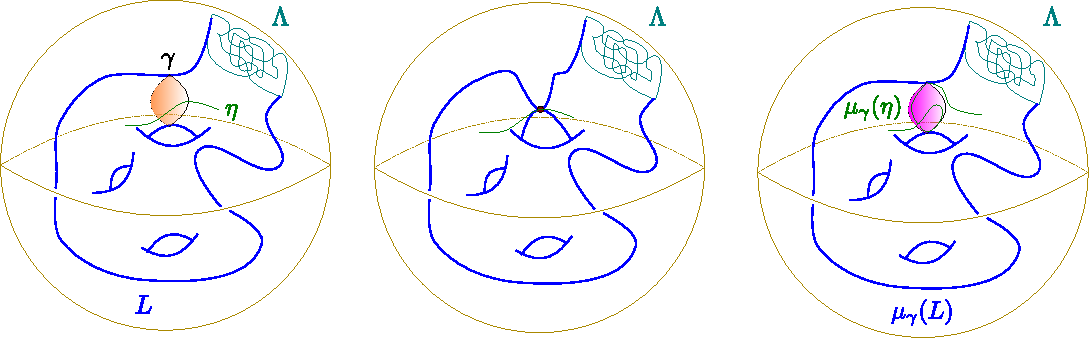
\includegraphics[width=\textwidth]{figures/Talks_CartoonSurgery.pdf}
		\caption{A Lagrangian filling $L\sse(\D^4,\la_\std)$ of a Legendrian link $(\La\sse \dd \D^4,\xi_\std)$ undergoing Lagrangian disk surgery. (Left) The Lagrangian disk $\D\sse \D^4\setminus L$ being surgered is depicted in orange, with boundary $\dd \overline{\D}=\gamma\sse L$. (Center) The critical moment of the surgery, where the filling $L$ degenerates to an immersed exact Lagrangian. (Right) The Lagrangian filling $\mu_\D(L)$, also denoted $\mu_\gamma(L)$, which is the result of the surgery. Here the new Lagrangian disk $\mu_\D(\D)\sse \D^4\setminus \mu_\g(L)$ after the surgery is depicted in purple, with boundary $\gamma\sse \mu_\g(L)$ oriented in reverse.}
		\label{fig:Talks_CartoonSurgery}
	\end{figure}
\end{center}

\begin{center}
	\begin{figure}[h!]
		\centering
		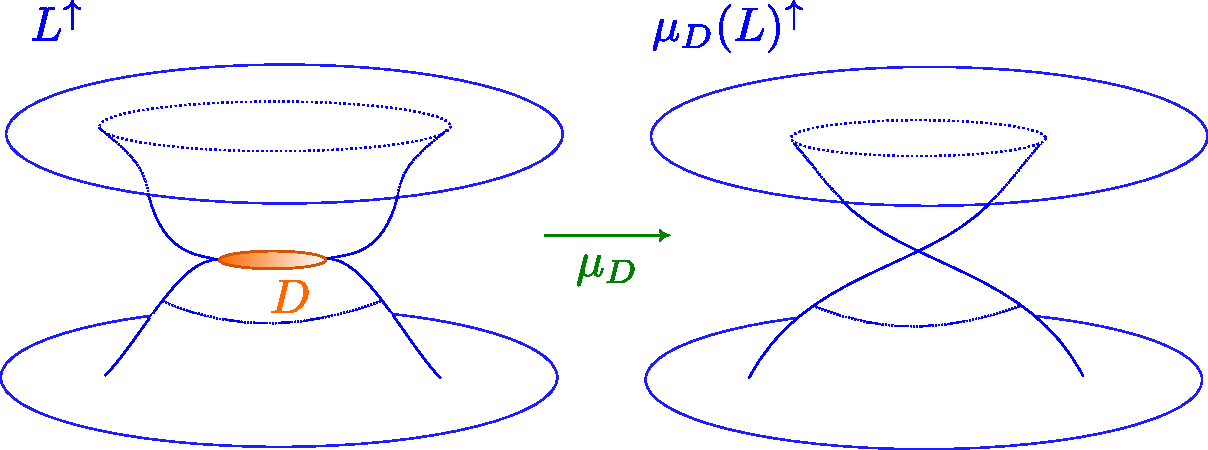
\includegraphics[scale=0.5]{figures/Surgery_InFront.pdf}
		\caption{The effect of Lagrangian disk surgery seen in fronts for the Legendrian lifts $L^\uparrow$ and $\mL^\uparrow$ of $L$ and $\mL$. These fronts can be understood in arbitrary dimensions, as spherical spins of the cusp, for the left front, and the cone point, for the right front. The disk $\D$, in orange, is the same disk in orange as in \cref{fig:Talks_CartoonSurgery} (Left) and a neighborhood of the cone point corresponds to a neighborhood of the purple disk in \cref{fig:Talks_CartoonSurgery} (Right).}
		\label{fig:Surgery_InFront}
	\end{figure}
\end{center}

\noindent L.~Polterovich introduced a beautiful construction in \cite[Sections 3\&4]{Polterovich_Surgery} that produces a (potentially) new Lagrangian filling $\mu_D(L)$ if one has an embedded Lagrangian disk $\D\sse \D^4\setminus L$ whose boundary $\dd\D\sse L$ belongs to $L$ as a clean intersection, i.e.~$\D\cap L=\dd\D$ and as transversely as possible. See also \cite[Section 3.3]{LalondeSikorav91_LagrangianSurgery} for the case of Lagrangian surfaces. This operation is local in a neighborhood of the disk $\D$, so the Lagrangian embeddings of $L$ and $\mu_D(L)$ coincide outside of a neighborhood of $\dd \D$. Intuitively, this operation can be depicted as in \cref{fig:Talks_CartoonSurgery}: the Lagrangian disk $\D$ is contracted to a point and expanded in a {\it different} way. It is proven in \cite[Theorem 1.1]{thomson2026legendrianhopflinkexactly} that there are only two ways to locally expand such contracted point, and thus this other expansion is locally unique. For a visualization locally around $\D$, the Legendrian lifts of $L$ and the surgered $\mu_D(L)$ can be represented via fronts as in \cref{fig:Surgery_InFront}. This is justified by the computations that now follow, cf.~also \cite[Section 6.2]{CasalsMurphyPresas}.\\

\begin{figure}
     \centering
     \begin{subfigure}[b]{0.4\textwidth}
         \centering
         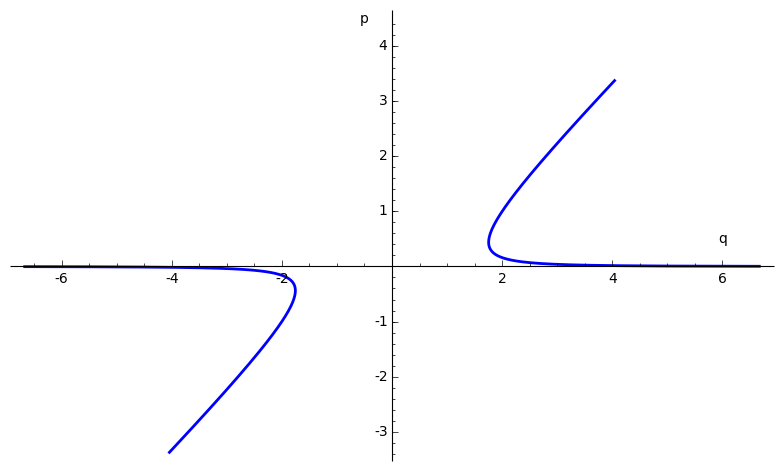
\includegraphics[width=\textwidth]{figures/CuspSum3_qp.png}
         \caption{Lagrangian handle $\Gamma^+$.}
         \label{fig:y equals x}
     \end{subfigure}
     %\hfill
     \begin{subfigure}[b]{0.4\textwidth}
         \centering
         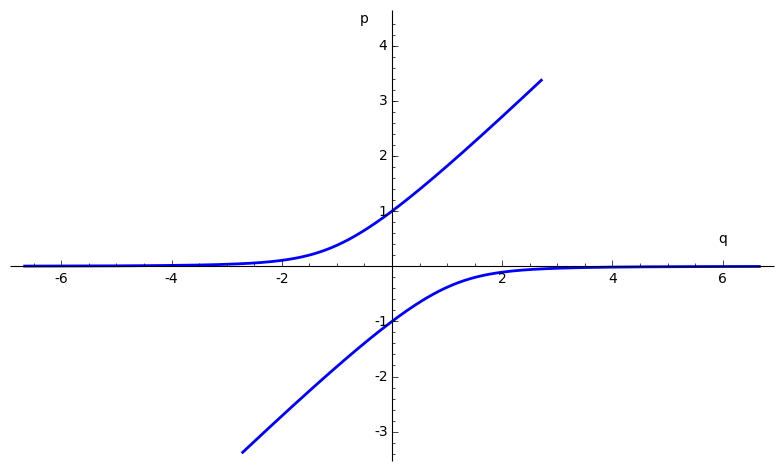
\includegraphics[width=\textwidth]{figures/ConeSum3_qp.png}
         \caption{Lagrangian handle $\Gamma^-$.}
         \label{fig:three sin x}
     \end{subfigure}
     \caption{The Lagrangian handles $\Gamma^{\pm}\subseteq\R^{2n}(q,p)$.}
     \label{fig:Lagr_handles}
\end{figure}

The local model for the Lagrangian surgery in \cite{Polterovich_Surgery} can be described as follows. Consider local coordinates $(q_1,q_2,p_1,p_2)\in\R^{4}$ and model the two sheets of an immersed point in a Lagrangian, as the one in \cref{fig:Talks_CartoonSurgery} (Center), and the Liouville form via
$$S_1:=\{p_1=0,p_2=0\},\quad S_2:=\{q_1=p_1,q_2=p_2\},\quad \displaystyle\lambda_\std=p_1dq_1+p_2dq_2.$$
The two Lagrangian handles $\Gamma^\pm$ presented in \cite{Polterovich_Surgery} provide two ways to resolve such an immersed point, resulting in an embedded exact Lagrangian. These Lagrangian handles are depicted in Figure \ref{fig:Lagr_handles}, and in order to explicitly parametrize them we use coordinates $t=(t_1,t_2)\in\R^{2}$. First, the positive Lagrangian handle $\Gamma^+$ can be described via the parametrization $\Gamma^+:\R^{2}\setminus\{0\}\longrightarrow\R^{4}$
defined as
$$\Gamma^+(t_1,t_2)=\left((\mu+\mu^{-1})t_1,(\mu+\mu^{-1})t_{2},\mu t_1,\mu t_{2}\right)\mbox{ where }\displaystyle\mu=t_1^2+t_2^2.$$

\noindent Note that $\Gamma^\pm$ are diffeomorphic to $S^{1}\times\R$, we have the two asymptotics
$$\displaystyle\lim_{\mu\to\infty}\Gamma^+\subseteq S_2,\quad \displaystyle\lim_{\mu\to0}\Gamma^+\subseteq S_1,$$
and in this model $L$ and $\D$ are described as follows:

\begin{enumerate}
    \item The given Lagrangian $L$ is obtained by gluing the above positive Lagrangian handle $\Gamma^+$ to the Lagrangian sheet $S_1$ at the limit $\mu=0$, and to the Lagrangian sheet $S_2$ at the limit $\mu=\infty$. Thus, intuitively, locally near the boundary $\dd\D\sse L$, the Lagrangian is modeled by $\Gamma^+$.\\

    \item The Lagrangian disk $\D$ is modeled within the Lagrangian graph $\Gamma_\ell$ of the linear function
    $$\ell:\R^2_{q_1,q_2}\lr\R^2_{p_1,p_2},\quad p_i=\frac{q_i}{2},\quad i\in[1,2].$$
    Specifically, $\D$ is the image of the restriction of $\Gamma_\ell$ to $\{\|q\|\leq2\}$.
    The boundary $\dd\D\sse L$ of $\D$ in this model can be taken to be the intersection $\Gamma_\ell\cap\Gamma^+$, which can be parametrized by $\Gamma^+(t_1,t_2)$ where $(t_1,t_2)\in S^1$ belong to the 1-sphere.\footnote{Note that, generically, two Lagrangian submanifolds intersect in points, not in codimension 1 subsets of each other. This model is {\it not} a generic situation and $\Gamma_\ell\cap\Gamma^+\cong S^{1}$ being diffeomorphic to a sphere does not persist under a generic Hamiltonian isotopy applied to either Lagrangian.}
\end{enumerate}

\noindent The surgered Lagrangian $\mu_\D(L)$ is obtained by using the negative Lagrangian handle $\Gamma^-:\R^2\setminus\{0\}\longrightarrow\R^{4}$ parametrized by
$$\Gamma^-(t_1,t_{2})=\left((\mu-\mu^{-1})t_1,(\mu-\mu^{-1})t_{2},\mu t_1,\mu t_{2}\right).$$
This parametrization satisfies the asymptotics $\displaystyle\lim_{\mu\to\infty}\Gamma^-\subseteq S_2$ and $\displaystyle\lim_{\mu\to0}\Gamma^-\subseteq S_1$, and can be glued to $S_1$ and $S_2$ in the asymptotic limits, thus constructing the Lagrangian $\mu_\D(L)$:

\begin{fdef}[Lagrangian disk surgery]\label{def:disk_surgery} In the local model above, the Lagrangian disk surgery of $L$ along $\D$ is the embedded exact Lagrangian $\mu_\D(L)$ obtained by exchanging the positive Lagrangian $\Gamma^+\sse L$ by the negative Lagrangian handle $\Gamma^-$.
\end{fdef}
\vspace{0.2cm}
\noindent This Lagrangian disk surgery in \Cref{def:disk_surgery} has the following properties:\\

\begin{enumerate}
    \item $\Gamma^+$ and $\Gamma^-$ are smoothly isotopic and thus $L$ and $\mu_\D(L)$ are smoothly isotopic. In fact, since $\Gamma^+$ and $\Gamma^-$ are even Lagrangian isotopic, so are $L$ and $\mu_\D(L)$.\\

    \item $\Gamma^+$ and $\Gamma^-$ are not Hamiltonian isotopic via a compactly supported Hamiltonian diffeomorphism of $\R^{4}$. Equivalently, $\Gamma^+$ and $\Gamma^-$ are not exact Lagrangian isotopic relative to their boundaries. This follows, for instance, from the fact that $\Gamma^\pm$ are Lagrangian fillings of the Hopf link inducing different augmentations, cf.~\cite[Section 8.1]{EHK}. Alternatively, and historically preceding ibid., this follows from the fact that the Chekanov and Clifford tori, which differ by a unique Lagrangian disk surgery, are not Hamiltonian isotopic, as proven in \cite[Section 4]{Chekanov96_Torus}.\\

    \item In the model above, the new Lagrangian 2-disk $\mu_\D(\D)$ is given by
    $$\mu_\D(\D):=\{(q,p)\in\R^{4}: q_1=0,q_2=0,\|p\|\leq1\},$$
    whose boundary $\dd\mu_\D(\D)$ is indeed contained in $\mbox{im}(\Gamma^-)$, as can be parametrized by $\Gamma^-(t_1,t_2)$ where $(t_1,t_2)\in S^{1}$ belong to the unit sphere.\\

    \item Lagrangian disk surgery is an involutive operation, in the sense that
    $$\mu_{\mu_\D(D)}(\mu_\D(L))\simeq L$$
    are Hamiltonian isotopic. This follows from the fact that, in the local model above, Lagrangian disk surgery applied to $\Gamma^-$ along $\mu_\D(\D)$ results in a Lagrangian which is Hamiltonian isotopic to $\Gamma^+$.\\

    \item It is natural to wonder whether there is a third way to resolve an immersed point, not just with $\Gamma^\pm$. It follows from \cite[Theorem 1.1]{thomson2026legendrianhopflinkexactly} that $\Gamma^\pm$ are the only embedded exact Lagrangian fillings of the Hopf link, up to Hamiltonian isotopy. Thus $\Gamma^\pm$ are the only two possible Lagrangian handles we could have constructed, up to Hamiltonian isotopy.\\
\end{enumerate}

%%%%%%%%%%%%%%%%%%%%%%%%%%%%%%%%%%%%%%%%%%%%%%%%%%%%%%%%
%%%%%%%%%%%%%%%%%%%%%%%%%%%%%%%%%%%%%%%%%%%%%%%%%%%%%%%%
%%%%%%%%%%%%%%%%%%%%%%%%%%%%%%%%%%%%%%%%%%%%%%%%%%%%%%%%
\subsubsection{Lagrangian disk surgery via weaves}\label{sssec:disk_surgery_via_weaves} 
The local model for Lagrangian disk surgery, as presented in \Cref{sssec:local_model_surgery}, can be realized as a weave mutation between Demazure weaves, as follows. Consider the singularity $P(z,w)=w^2-z^2$ and, following \Cref{ssec:Lagrangian_filling_from_AG}, we can consider the two real Morsifications:
\begin{equation}\label{eq:Lagrangian_surgery_models}
P_\pm(z,w):=w^2-z^2\pm1,\qquad L_\pm:=\{(z,w)\in\C^2:w^2-z^2\pm1=0\}
\end{equation}
\noindent As in \Cref{lem:complex_curve_real_Lagrangian}, each $L_\pm$ provides a real Lagrangian cylinder in $(\R^4,\la_\std)$ and each is exact, since the residue formula implies that the unique period of $zdw-wdz$ on each of $L_\pm$ is an integer multiple of $2\pi i$. The graphs of the fronts of their Legendrian lifts of $L_\pm$ are depicted in \Cref{fig:Graphs_weave_mutation}, along with that of the immersed Lagrangian $\{P(z,w)=0\}$.

\begin{center}
	\begin{figure}[h!]
		\centering
		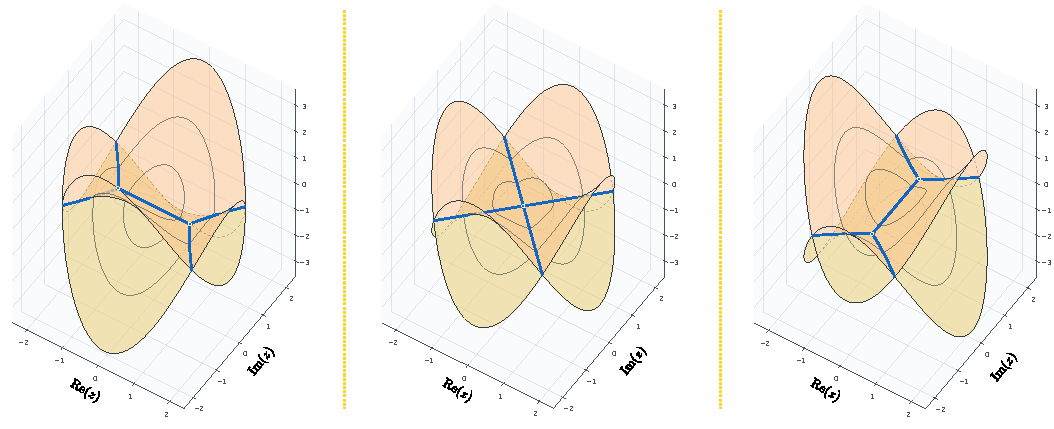
\includegraphics[width=\textwidth]{figures/Graphs_weave_mutation.pdf}
		\caption{(Left) The weave, inside the corresponding 3-dimensional graph, associated to the exact Lagrangian cylinder $L_+$ from \eqref{eq:Lagrangian_surgery_models}. (Center) The weave corresponding to the immersed exact Lagrangian $\{w^2-z^2=0\}$. (Right) The weave associated to the exact Lagrangian cylinder $L_-$ from \eqref{eq:Lagrangian_surgery_models}.}
		\label{fig:Graphs_weave_mutation}
	\end{figure}
\end{center}

\noindent An $\L$-compressing disk $\D_\pm\sse\R^4\setminus L_\pm$ for each of $L_\pm$ can be described as follows:\\

\begin{enumerate}
    \item Consider the embedded 2-disk
    \begin{equation}\label{eq:compressing_disk_MorsificationA1_plus}
    \begin{split}
    \D_+&:=\left\{(z,w)\in\C^2: \Re(z)\in[-1,1],\Im(z)=0, w\in\left[-\sqrt{z^2-1},\sqrt{z^2-1}\right]\right\}\cong\\
        &=\{(x,iy):x,y\in\R,x^2+y^2\leq 1\}
        \end{split}
    \end{equation}
    which is Lagrangian and, by construction, $\dd\D_+\sse L_+$ provides a representative for the generator of $\hH_1(L_+,\Z)$. The associated weave $\w_+$ is depicted in \Cref{fig:Graphs_weave_mutation} (left), and it has trivalent vertices at $z=\pm1$ with the only mutable Lusztig cycle being supported at the segment $\Re(z)\in[-1,1]$ with $\Im(z)=0$. Note that the projection of $\D_+$ to $\R^2_{x_1,x_2}\cong\C_z$ is indeed given by this Lusztig cycle.\\
    
    \noindent Compressing the Lagrangian 2-disk $D_+$ as in \Cref{sssec:local_model_surgery} leads to the immersed Lagrangian $\{P(z,w)=0\}\cong \C_{\{z=w\}}\cup \C_{\{z=-w\}}\sse\C^2$, which has a unique (immersed) singular point at the origin. The front for its Legendrian lift is drawn in \Cref{fig:Graphs_weave_mutation} (center). This degeneration, given by compressing the disk, can be performed through exact Lagrangians by introducing a real parameter $\alpha\in(0,1]$ in \eqref{eq:Lagrangian_surgery_models} and considering the exact Lagrangian surfaces $\{w^2-z^2+\alpha=0\}$ from $\alpha=1$ to $\alpha=0$.\\

     \item Similarly, we can consider the embedded 2-disk
    \begin{equation}\label{eq:compressing_disk_MorsificationA1_plus2}
        \begin{split}
        \D_-&=:=\left\{(z,w)\in\C^2: \Re(z)=0,\Im(z)\in[-1,1], w\in\left[-\sqrt{z^2+1},\sqrt{z^2+1}\right]\right\}\\
                &=\{(ix,y):x,y\in\R,x^2+y^2\leq 1\}
        \end{split}
    \end{equation}
    which is an exact Lagrangian disk with $\dd\overline{\D}_-\sse L_-$. As above, the projection of $\D_-$ to $\R^2_{x_1,x_2}\cong\C_z$ is given by the Lusztig cycle \{$\Re(z)=0,\Im(z)\in[-1,1]$\} associated to the weave $\w_-$ for $L_-$. The two trivalent vertices of such a weave are located at $z=\pm i$, as illustrated in \Cref{fig:Graphs_weave_mutation} (right). Compressing $D_-$ as in \Cref{sssec:local_model_surgery} can be realized similarly via the exact Lagrangian surfaces $\{w^2-z^2-\alpha=0\}$ where $\alpha\in[0,1]$ is a real parameter.\\
\end{enumerate}


In conclusion, the Lagrangian disk surgery, as described in \Cref{sssec:local_model_surgery}, can be locally modeled by the transition from one of the two sides of \Cref{fig:Graphs_weave_mutation} to the other, through the center model. Thus we obtain

\begin{equation}\label{eq:mutation_via_fillings}
       \mu_{\D_+}(L_+)\simeq L_-\qquad\&\qquad\mu_{\D_-}(L_-)\simeq L_+
\end{equation}

\noindent In combination with \Cref{fig:Graphs_weave_mutation}, \eqref{eq:mutation_via_fillings} geometrically justifies that the diagrammatic weave mutation from \Cref{fig:weave_mutation} (left) is diagrammatically encoding a Lagrangian disk surgery. Namely, if $\w_+$ and $\w_-$ are the only two weaves $\w_\pm:\s_1^3\lr\s_1$, \Cref{fig:weave_mutation} (left), which differ by a weave mutation, then:

        \begin{equation}\label{eq:mutation_via_fillings}
        \fbox{$\mu_{\D_+}(L_{\w_+})\simeq L_{\w_-}\quad\&\quad \mu_{\D_-}(L_{\w_-})\simeq L_{\w_+}$}
        \end{equation}

\noindent This geometric realization of weave mutation, with $L_\pm$ not being Hamiltonian isotopic, was a strong reason to define weave mutation as we did in \Cref{def:weave_mutation}.

\begin{remark}
It follows from the local model above that $L_\pm$ are actually compactly supported smoothly isotopic to each other. In particular, their relative homology classes coincide. This explains why in diagrammatic Soergel calculus, cf.~\cite{EliasWilliamson2016Calculus,EMTW2020}, the move \Cref{fig:weave_mutation} (left) is instead considered an equivalence. Indeed, in Soergel calculus only the homology classes of these surfaces are relevant as a Hochschild homology is being taken, cf.~\cite{Webster_2008}.\sbs
\end{remark}

%%%%%%%%%%%%%%%%%%%%%%%%%%%%%%%%%%%%%%%%%%%%%%%%%%%%%%%%%%%%%%%%%
%%%%%%%%%%%%%%%%%%%%%%%%%%%%%%%%%%%%%%%%%%%%%%%%%%%%%%%%%%%%%%%%%

\subsubsection{$\L$-compressing systems}\label{sssec:L_compressing_systems} Let $\La\sse(T^\infty\R^2,\xi_\std)$ be a Legendrian link and $L\sse (T^*\R^2,\la_\std)$ a Lagrangian filling. We can try to apply Lagrangian disk surgeries to $L$, as discussed in \cref{sssec:local_model_surgery}, to produce Lagrangian fillings that are potentially new, i.e.~not Hamiltonian isotopic to $L$. The input of a Lagrangian disk surgery is $L$ and an embedded Lagrangian disk $\D\sse\D^4\setminus L$ with $\dd\overline{D}\sse L$. The next question thus becomes: \textcolor{blue}{given a Lagrangian $L$, how do we find such embedded Lagrangian 2-disks $\D$}?\\

\noindent The short answer is that this is not known in general. We will nevertheless present many interesting cases, some connected to singularity theory and some to algebraic combinatorics, in which these disks appear naturally. In order to have a precise language to talk about these situations, we introduce the following notion:

\begin{fdef}[$\L$-compressing systems]\label{def:Lcompressing_systems} Let $L\sse (\D^4,\la_\std)$ be a Lagrangian filling of $\dd L\sse(S^3,\xi_\std)$. By definition, an $\L$-compressing system $\D(L):=\{\D_1,\ldots,\D_s\}$ of rank $s$ is a collection of disks $\D_i\sse \D^4\setminus L$, $i\in[1,s]$, such that\\
\begin{enumerate}
    \item $\D_i$ is an embedded Lagrangian disk with $\dd\overline{\D_i}\sse L$ a clean intersection, for all $i\in[1,s]$,\\
    \item The collection of boundary classes $\{\dd\overline{\D_1},\ldots,\dd\overline{\D_s}\}$ is linearly independent in $H_1(L)$.\\
\end{enumerate}
By definition, an $\L$-compressing system $\D(L):=\{\D_1,\ldots,\D_s\}$ is said to be maximal if the boundaries of the disks $\D_i\in\D(L)$ span $H_1(L,\Z)$.\sbs
\end{fdef}
\vspace{0.2cm}
\noindent A given Lagrangian $L\sse (\D^4,\la_\std)$ might not admit a maximal $\L$-compressing system. To wit, the Legendrian representative of $m(5_2)$ in \cref{fig:Front_Arc_Cusp_Crossing_R3_Example1} (left) has two known distinct embedded Lagrangian fillings, both once-punctured tori: both of them admit an $\L$-compressing system of rank 1, but neither of them admits an $\L$-compressing system of rank 2. There are relaxations of \cref{def:Lcompressing_systems}, allowing for {\it immersed} Lagrangian disks, cf.~\cite[Section 3]{CasalsWeng22}, but we focus on maximal $\L$-compressing systems in this manuscript.

\begin{remark} (1) \cref{def:Lcompressing_systems} naturally generalizes to embedded exact Lagrangians $L\sse (\D^4,\la_\std)$ in a Liouville manifold $(W,\la_\std)$ by using the concept of relative Lagrangian skeleton. For instance, a maximal $\L$-compressing system for a given $L\sse(\D^4,\la_\std)$ is a collection $\D(L)$ of embedded Lagrangian disks $\D_i\sse \D^4\setminus L$, $i\in[1,s]$, with $\dd\overline{D_i}\sse L$ such that
$$L\cup(\D_1\cup\ldots\D_s)$$
is a relative Lagrangian skeleton of $(\D^4,\la)$, relative to the Weinstein hypersurfaces given by the Weinstein ribbon of $\dd L\sse\dd\D^4$. In the case of $(W,\la)\cong (\D^4,\la_\std)$, this generalizes the condition of $\{\dd\D_1,\ldots,\dd\D_s\}$ being a basis of $H_1(L,\Z)$.\\

\noindent (2) It is oftentimes useful to relax the condition that the boundary homology classes of the disks $\D_i$ are linearly independent. This case is particularly relevant in the study of Landau-Ginzburg models which appear on the B-side of the homological mirror symmetry correspondence for Fano varieties, see e.g.~\cite{PascaleffTonkonog20}.\sbs
\end{remark}

\begin{example}\label{ex:Lcompressing_systems} (1) The Legendrian links $\La(\bG)$ associated to plabic graphs $\bG$, as the lifts of their alternating strand diagram, come endowed with both a Lagrangian filling {\it and} an $\L$-compressing system. Intuitively, the $\L$-compressing system is given by the bounded faces of $\bG$, understood as Lagrangian disks in the zero section. See e.g.~\cite[Section 4.3]{CasalsGao24}, and see \cite[Section 3]{casals2023demazureweavesreducedplabic} for their relationship to Demazure weaves $\w$ and their Lagrangian fillings $L_\w$. These $\L$-compressing systems are maximal in many interesting cases, e.g.~for reduced plabic graphs.\\

\noindent (2) Given an isolated plane curve singularity $f:\C^2\lr\C$ with a real Morsification, the Lagrangian fillings from \cref{ex:Lagrangian_fillings}.(3) come endowed with a maximal $\L$-compressing system. The Lagrangian disks are provided by the Lefschetz thimbles, and their boundary curves in the Lagrangian Milnor fiber are the vanishing cycles, cf.~\cite[Section 2]{CasalsLagSkel}.\sbs
\end{example}

%%%%%%%%%%%%%%%%%%%%%%%%%%%%%%%%%%%%%%%%%%%%%%%%%%%%%%%%%%%%%%%%%
%%%%%%%%%%%%%%%%%%%%%%%%%%%%%%%%%%%%%%%%%%%%%%%%%%%%%%%%%%%%%%%%%

\subsubsection{$\L$-compressing systems from Demazure weaves}\label{sssec:L_compressing_systems_via_weaves} Let $\wb$ be a Demazure weave and $\g_i^\w$ a mutable Lusztig cycle. If we want to geometrically realize the weave mutation $\w\stackrel{\mu}{\sim}\w'$ via a Lagrangian disk surgery we must find a Lagrangian 2-disk $\D_i\sse\D^4\setminus L_\w$ in the complement of $L_\w$ whose boundary represents the homology class $\g_i^\w$. Recall that $L_\w\sse\D^4$ is embedded in a way that the restriction of the projection
$$\pi:\D^4\lr\R^2$$
to $L_\w$ induces a simple branched cover $\pi|_{L_\w}:L_\w\lr\R^2$, for which the weave $\w$ acts as a branch cut. In the same manner that we associated a curve in $L_\w$ to a Lusztig cycle $\g_i^\w$ by using this branched cover, cf.~\Cref{sssec:X_lattice}, we can in many cases find such 2-disk $\D_i$ in a way that it maps to the support of the Lusztig cycle $\g_i^w$. Specifically, let us consider Lusztig cycles $\g_i^\w$ whose weights are either 0 or 1 and whose support in $\w$ is a tree, seen as a graph. Such weave cycles are referred to as $\mathsf{Y}$-cycles, cf.~\cite{CasalsWeng22,CasalsZaslow}. For these Lusztig cycles one obtains the following first result:

\begin{proposition}[$\L$-compressing 2-disk above a Lusztig $\mathsf{Y}$-cycle]\label{prop:compressing_disk_Lusztig_cycle}
Let $\wb$ be a Demazure weave, $L_\w\sse(\R^4,\la_\std)$ its associated Lagrangian filling, and $\g_i^\w$ a mutable Lusztig $\mathsf{Y}$-cycle. Then there exists a properly embedded Lagrangian 2-disk $\D_i\sse\R^4\setminus L_\w$ such that:\\
\begin{enumerate}
    \item $[\dd\D_i]=[\g_i^\w]$ and, after applying a sequence of weave equivalences to $\w$, the image $\pi(\D_i)$ coincides with the support of the corresponding Lusztig cycle $\g_i^\w$.\\

    \item The Lagrangian disk surgery of $\L_w$ along $D_i$ is Hamiltonian isotopic to $L_{\mu_i(\w)}$, i.e.~
        \begin{equation}\label{eq:mutation_via_fillings2}
        \fbox{$\mu_{\D_i}(L_\w)\simeq L_{\mu_i(\w)}$}
        \end{equation}
    where $\mu_i(\w)$ denotes the weave mutation of $\w$ at $\g_i^\w$.\sbs
\end{enumerate}
\end{proposition}

\noindent The simplest instance of \Cref{prop:compressing_disk_Lusztig_cycle}, and one of the ingredients for its proof, is the local model for Lagrangian disk surgery, presented in \Cref{sssec:local_model_surgery}, as realized via weaves in \Cref{sssec:disk_surgery_via_weaves}. Indeed, the two Lagrangian 2-disks $\D_\pm$ in \eqref{eq:compressing_disk_MorsificationA1_plus} and \eqref{eq:compressing_disk_MorsificationA1_plus2} project exactly over the unique Lusztig cycle for the corresponding Demazure weaves $\w:\s_1^3\lr\s_1$.\sbs \\

In general, it is an interesting question whether one can iterate such Lagrangian disk surgeries. For instance, given a mutation sequence (e.g.~by naming a sequence of vertices in the quiver $Q_\w$), the question is whether it is possible to geometrically realize it by iterated Lagrangian disk surgeries. At its core, this problem reduces to a question of algebraic intersection numbers, which are tracked by the arrows of the quivers, and geometric intersection numbers. Intuitively, if these algebraic and geometric intersection numbers coincide, then iterating is possible.\\

A study of this phenomenon can be found in \cite{CasalsGao24}, where it is shown that any cluster seed in $\Z[X(\beta)]$ can be obtained as the seed associated to a Lagrangian filling, as stated in Theorem \ref{thm:symplectic_intro2}. The proof shows that it is possible to geometrically iterate, using Lagrangian disk surgeries, such algebraic sequences of quiver mutations. The key idea is to introduce a potential $W_\w$ for $Q_\w$ that keeps track of the difference between the algebraic and geometric intersection numbers and show that such a quiver with potential is non-degenerate. In fact, it is proven in ibid.~that the quiver with potential $(Q_\w,W_\w)$ is rigid. From a symplectic topological perspective, the quiver with potential $(Q_\w,W_\w)$ encodes the $A_\infty$-structure for the union of all the exact Lagrangian curves in the symplectic push-off of the Lagrangian filling $L_\w$. In a sense, such a union can be seen as a collection of vanishing cycles and, being in a symplectic surface, all the relevant pseudo-holomorphic disk contributions can be combinatorialized in terms of polygons, as presented in \cite[Section 2]{CasalsGao24}.

%%%%%%%%%%%%%%%%%%%%%%%%%%%%%%%%%%%%%%%%%%%%%%%%%%%%%%%%%%%%%%%%%
%%%%%%%%%%%%%%%%%%%%%%%%%%%%%%%%%%%%%%%%%%%%%%%%%%%%%%%%%%%%%%%%%
%{\bf EDITED TILL HERE\\}

%%%%%%%%%%%%%%%%%%%%%%%%%%%%%%%%%%%%%%%%%%%%%%%%%%%%%%%%
%%%%%%%%%%%%%%%%%%%%%%%%%%%%%%%%%%%%%%%%%%%%%%%%%%%%%%%%
%%%%%%%%%%%%%%%%%%%%%%%%%%%%%%%%%%%%%%%%%%%%%%%%%%%%%%%%
%\subsection{Summary of section}

